\chapter{Methodik}
\label{chap:methodik}
Die Methodik dieser Arbeit beschreibt die wissenschaftlichen Hintergründe für das Vorgehen der Implementierung des Dashboard in einer \gls{dfir}-Umgebung für Open RAN. Der Fokus liegt auf der Integration von \gls{acema} und der (Weiter-)Entwicklung passender Visualisierungstechniken. Im Methodikteil werden die wissenschaftlichen Hintergründe über getroffene Entscheidungen erläutert. Zudem werden die Herausforderungen und Einschränkungen bei der Anwendung der Methoden reflektiert, um die Validität der Forschung kritisch zu beleuchten.
\section{Auswahl der empirischen Methode}
\label{sec:auswahlDerEmpirischenMethode}
\gls{acema} ist \glqq eine umfassende empirische Methode zur Analyse von Bedrohungen in O-RAN Umgebungen \grqq (eigene Übersetzung: \autocite{klementSecuring6GTransition2024}). Die Integration von \gls{acema} in das Forschungsprojekt \gls{foran} bringt umfangreiche Daten ein, die nützliche Visualisierungen im Dashboard ermöglichen. Im Folgenden wird erläutert, welchen Mehrwert \gls{acema} für \gls{foran} bietet und wie die gewonnen Daten angemessen im Dashboard visualisiert werden könne.
\par 

%
\begin{figure}[H]
    \centering
    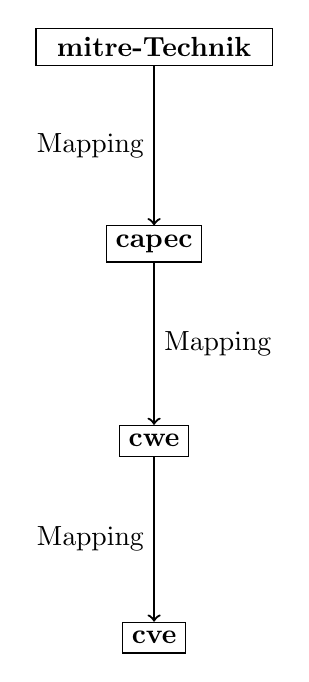
\begin{tikzpicture}[node distance=2cm, auto]
        % Nodes
        \node [rectangle, draw, text centered, minimum width=3cm] (mitre) {\textbf{\gls{mitre}-Technik}};
        \node [rectangle, draw, below of=mitre, yshift=-0.5cm] (capec) {\textbf{\gls{capec}}};
        \node [rectangle, draw, below of=capec, yshift=-0.5cm] (cwe) {\textbf{\gls{cwe}}};
        \node [rectangle, draw, below of=cwe, yshift=-0.5cm] (cve) {\textbf{\gls{cve}}};
        % Arrows
        \draw[->, thick] (mitre) -- (capec) node[midway, left] {Mapping};
        \draw[->, thick] (capec) -- (cwe) node[midway, right] {Mapping};
        \draw[->, thick] (cwe) -- (cve) node[midway, left] {Mapping};
    \end{tikzpicture}
    \caption{Abbildung einer \gls{mitre}-Technik zu einem spezifischen CVE-Datum über die Kategorisierungssysteme \gls{mitre}, \gls{capec}, \gls{cwe} und \gls{cve}.}
    \label{fig:mitre_mapping}
\end{figure}

\section{Datenquellen}
\label{sec:datenquellen}
\section{Auswahl der Visualisierungstechniken}
\label{sec:auswahlDerVisualisierungstechniken}
Die Basis für die Wahl der Visualisierungstechniken im Dashboard wurden von Jonas Weber in seiner Arbeit \citetitle{weberEvaluationDashboardTechniques} gelegt. \citeauthor{weberEvaluationDashboardTechniques} beschreibt darin grundlegende Prinzipien, die beim Design eines Dashboard eine wichtige Rollen spielen.
\par Das erste Prinzip beschreibt das Phänomen der präattentiven Wahrnehmung. Darunter versteht man die Wahrnehmung von visuellen Reizen, welches jedoch unterschwellig und ohne das Dazutun von Aufmerksamkeit passiert. Man spricht auch von Vorbewusstsein \autocite{PrC3A4attentiveWahrnehmung}, \autocite{mallotWahrnehmungPraeattentiveIm2021}. Über das Design von Dashboard auf Basis dieses neurologischen Konzept gibt es zahlreiche Wissenschaftliche Arbeiten, hervorgehoben sei dabei die Übersicht von \autocite{barrera-leonHowPreattentiveProcess2023} mit dem Titel \citetitle{barrera-leonHowPreattentiveProcess2023} \autocite{barrera-leonHowPreattentiveProcess2023}. Anwendung findet dieses Prinzip in der Implementierung des Dashboards zum Beispiel beim Design der Zeitleiste. In Abbildung \ref{fig:cvss-colors} ist dargestellt, wie der Schweregrad von Metriken eines \gls{cve}'s anhand einer farblichen Kategorisierung eingeordnet wird. Die Farbwahl beschränkt sich hierbei auf vier deutlich voneinander unterscheidbaren Farben \todo{Hier eventuell als Tabelle oder textit oder so...}: Grau für Keine Daten vorhanden, Grün für Niedriger Schweregrad, Gelb für Mittlerer Schweregrad, Rot für Hoher Schwerergrad. Wissenschaftlich ist die kategorische Wahrnehmung von Farben unter anderem durch die wissenschaftliche Arbeit von \citeauthor{cliffordColorCategoriesAffect2010} bewiesen \autocite{cliffordColorCategoriesAffect2010}. Die technische Implementierung der Farbkategorisierung ist in Kapitel \ref{sec:cvssIntegration} erläutert.
%
\begin{figure}[H]
    \centering
    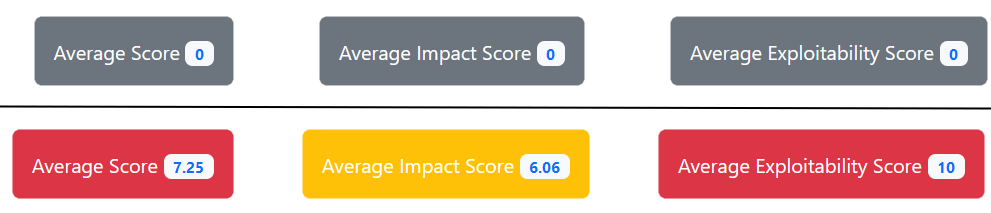
\includegraphics[width=0.8\textwidth]{cvss-colors}
    \caption{Farbkategorien zur Darstellung von Metriken}
    \label{fig:cvss-colors}
\end{figure}
%
\par \todo{In diesem Kapitel Lit-Verweise einfügen!!!} Ein weiteres Prinzip, welches beim Visualisieren von Daten eine zentrale Bedeutung hat wurde 1983 von \citeauthor{tufteBookReviewsVisual1984} als \textit{data-ink}-Prinzip definiert. Das Prinzip besagt, dass der Anteil der genutzten Farbe um die Daten darzustellen möglichst hoch sein soll. Damit soll die Darstellung von nicht-daten-bezogener \glqq Ausschönung \grqq in der Visualisierung vermieden werden. An einem praktischen Beispiel kann jedoch gezeigt, dass ein geringeres \textit{data-ink} Verhältnis nötig sein kann, um Daten effizient darzustellen. In Kapitel \ref{sec:tech-foran} ist der Dateninhalt eines Artefaktes beschrieben. Als zentrale zu visualisierende Daten liegen jeweils das Start- und Enddatum der Artefakte vor. Die Abbildung \ref{fig:high-data-ink} zeigt die Darstellung von mehreren Artefakten auf einer Zeitleiste. Das \textit{data-ink} Verhältnis ist in dieser Darstellung sehr hoch, da tatsächlich nur die Start- und Endzeitpunkte dargestellt sind. In \ref{fig:low-data-ink} ist die Zeitspanne zwischen den jeweiligen Daten eines Artefaktes farblich dargestellt. Es wird erkennbar, welche Punkte Start- oder Endpunkte sind. Dies war in Abbildung \ref{fig:high-data-ink} nicht intuitiv erkenntlich. Es ist in diesem Fall sinnvoll ein niedriges \textit{data-ink} Verhältnis zu erzielen, um Klarheit und Intuition zum Lesen zu schaffen. Die technische Konfiguration der Zeitleiste ist in Kapitel \todo{In welchem Kapitel kann ich darüber reden, aktuell passt keins...} erläutert.
%
\begin{figure}[H]
    \centering
    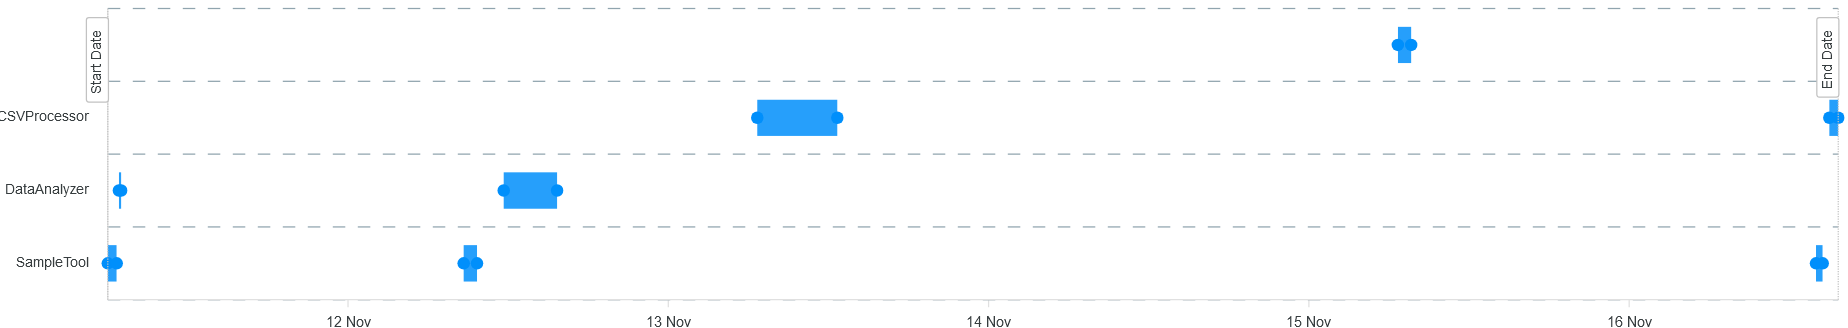
\includegraphics[width=1\textwidth]{low-data-ink}
    \caption{Niedriges \textit{data-ink} Verhältnis}
    \label{fig:low-data-ink}
\end{figure}
%
\begin{figure}[H]
    \centering
    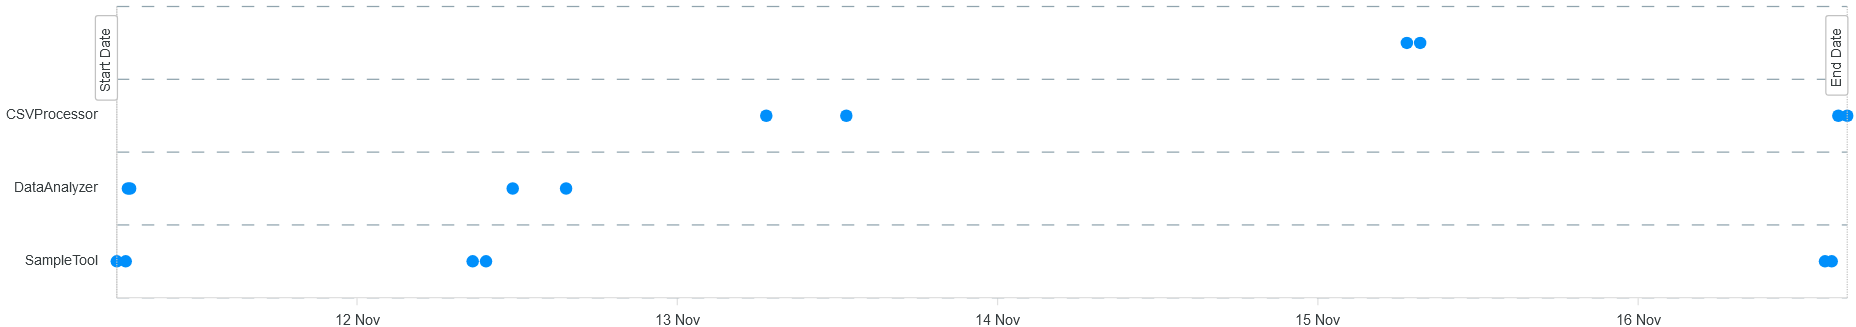
\includegraphics[width=1\textwidth]{high-data-ink}
    \caption{Hohes \textit{data-ink} Verhältnis}
    \label{fig:high-data-ink}
\end{figure}
%
\par Diese beiden Prinzipien und \textit{best-practices} wurden auch bei Weiter- und Neuentwicklungen bei Visualisierung im Dashboard gewahrt. Bei der Darstellung des Angriffspfads und der Netzwerktopologie wurden bewusste designtechnische Entscheidungen getroffen. Was genau unter diesen beiden neuen Visualisierungen zu verstehen ist, wurde in Kapitel \ref{sec:tech-foran} \todo{Oder leicht woanders, wenn es dort noch weitere Unterkapitel gibt.} bereits definiert. Die Angriffspfads-Visualisierung enthält nicht viele Daten, nimmt aber einen großen Platz auf der Detailübersicht eines Artefaktes ein. Der Angriffsgraph und Netzwerkgraph sind beim Laden der Seite nicht direkt, sondern nur nach einem bewussten Scrollen sichtbar. So wird der Nutzer nicht mit zu vielen Informationen auf einmal überladen. Die Graphen werden nicht als statische Bilder eingebettet. So lassen sich weitere Funktionen wie Tooltipps, dynamischer Zoom und die Verschiebbarkeit der einzelnen Elemente realisieren. Ein Tooltip hat hier die Funktion, zusätzliche hilfreiche Information zu liefern wenn der Nutzer mit dem Mauszeiger auf ein Element zeigt \autocite{TooltipCarbonDesign}. Die Implementierung des Tooltip ist in Abbildung \ref{fig:tooltip} gezeigt. Über die Verschiebbarkeit der Elemente kann das Diagram angepasst werden, um es verständlicher darzustellen oder für einen Export vorzubereiten. Die Graphen können über gängige Browser per \textit{Rechtsklick, Speichern unter / In neuem Tab öffnen} als \verb|.png| Datei exportiert werden.
%
\begin{figure}[H]
    \centering
    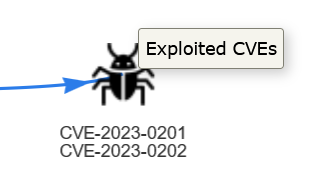
\includegraphics[width=0.5\textwidth]{tooltip}
    \caption{Tooltip auf einem Element im Angriffsgraphen}
    \label{fig:tooltip}
\end{figure}
%
\par Ausschnitte über die Implementierung im Quellcode der Graphen sind in Kapitel \ref{sec:visualisierungDesAngriffspfads} gezeigt.
\section{Entwicklungsumgebung}
\label{sec:Entwicklungsumgebung}
Ich gehe in diesem Kapitel etwas tiefer auf die Tools ein, die ich zur Umsetzung der Implementierung des Dashboard genutzt habe. Die generelle Architektur, genutzte Programmiersprachen und Technologien findet sich in Kapitel \ref{sec:tech-dashboard}. Zu Beginn wurde die Entwicklung auf einer rein lokalen Umgebung durchgeführt. Über das von MongoDB zur Verfügung gestellte \gls{cli} lief ein MongoDB-Server, ein per \verb|go build| gebaute Dashboard-Server und der per \verb|yarn dev| gestartete Vite-Entwicklungs-Server auf dem lokalen Rechner \autocite{MongoDBDeveloperData} \autocite{Vite}. Die Testdaten stammten aus dem Gitlab-Repo und sind von Jonas Weber zur Verfügung gestellt \autocite{AddExampleData2023}. Die Qualität und Menge der Testdaten war für den Anfang ausreichen. Um auf aktuellen Daten zu arbeiten und näher an der etablierten Testumgebung zu sein, nutzte ich ab dem 7. August 2024 eine \gls{vm} in der \glqq\gls{dnlab}\grqq-Umgebung der TH Köln. Das Arbeiten auf einem entfernten (\textit{en: remote}) Host innerhalb von \gls{vscode} wird seit 2019 durch eine von Microsoft entwickelte Erweiterung vereinfacht \autocite{RemoteSSHVisual}. Die Anwendung kann dann entweder weiterhin lokal auf der \gls{vm} oder zentralisiert per Ansible bereitgestellt (\textit{en: deployed}) werden \autocite{HomepageAnsibleCollaborative}. Ansible ist ein Tool zur Orchestrierung von Systemen und Software, welches durch die Ausführung von Skripten einen spezifischen technischen Zustand herstellt \autocite{alHowAnsibleWorks2024}. Auf die Entwicklung der Deployment-Skripte für die automatisierte Bereitstellung der Dashboard Komponente in der \gls{foran}-Umgebung der TH Köln und PROCYDE gehe ich in Kapitel \todo{Hier Kapitel Nr einfügen.} genauer ein.
\par Für die Ausführung des \gls{acema}-Quellcodes ist das Aufsetzen einer Python-Umgebung nötig \autocite{FklementAcema_oranCode} \autocite{WelcomePythonorg}.
\section[Einschränkungen]{Einschränkungen von ACEMA}
\label{sec:einschränkungen}